% ------------------------------------------------------------------------------
% TYPO3 CMS 6.2 LTS - What's New - Chapter "Introduction" (German Version)
%
% @author	Michael Schams <schams.net>
% @license	Creative Commons BY-NC-SA 3.0
% @link		http://typo3.org/download/release-notes/whats-new/
% @language	German
% ------------------------------------------------------------------------------
% Chapter: Introduction
% ------------------------------------------------------------------------------

\section{Einführung}
\begin{frame}[fragile]
	\frametitle{Einführung}

	\begin{center}\huge{Einführung}\end{center}
	\begin{center}\huge{\color{typo3darkgrey}\textbf{(Die Fakten)}}\end{center}

\end{frame}

% ------------------------------------------------------------------------------
% TYPO3 CMS 6.2 LTS: The Facts (1)
% ------------------------------------------------------------------------------

\begin{frame}[fragile]
	\frametitle{Einführung}
	\framesubtitle{TYPO3 CMS 6.2 LTS: Die Fakten}

	\begin{itemize}
		\item Hauptziele:

			\begin{itemize}
				\item Reibungslose Migration
				\item Robuste und sichere Grundlage
				\item Hohe Benutzerakzeptanz
				\item Moderne Technologien/Interoperabilität
			\end{itemize}

	\end{itemize}

	\begin{columns}[T]

		\begin{column}{.5\textwidth}
			\begin{itemize}
				\item Release Manager:
				\begin{itemize}
					\item Ernesto Baschny\newline
						ernesto.baschny (at) typo3.org\newline
						Twitter: @baschny
				\end{itemize}
			\end{itemize}
		\end{column}

		\begin{column}{.5\textwidth}
			\begin{figure}
				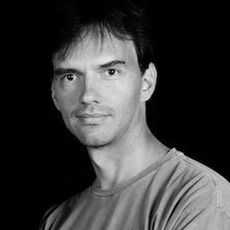
\includegraphics[width=2.6cm,height=2.6cm]{Images/Introduction/ErnestoBaschny.jpg}
			\end{figure}
		\end{column}

	\end{columns}

\end{frame}

% ------------------------------------------------------------------------------
% TYPO3 CMS 6.2 LTS: The Facts (2)
% ------------------------------------------------------------------------------

\begin{frame}[fragile]
	% \TabPositions{1.2cm}

	\frametitle{Einführung}
	\framesubtitle{TYPO3 CMS 6.2 LTS: Die Fakten}

	\begin{itemize}
		\item Veröffentlichungsdatum: 25 März 2014
		\item Entwicklungs- und Veröffentlichungszeitplan:
	\end{itemize}

	\begin{figure}
		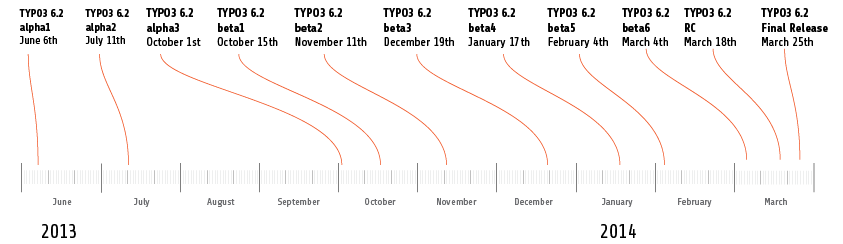
\includegraphics[width=0.99\linewidth]{Images/Introduction/ReleaseTimeline.png}
	\end{figure}

\end{frame}

% ------------------------------------------------------------------------------
% TYPO3 CMS 6.2 LTS: The Facts (3)
% ------------------------------------------------------------------------------

\begin{frame}[fragile]
	\frametitle{Einführung}
	\framesubtitle{TYPO3 CMS 6.2 LTS: Die Fakten}

	\begin{itemize}
		\item Systemvoraussetzungen
		\begin{itemize}
			\item PHP	\tabto{1.2cm} v5.3.7 - v5.5.x
			\item MySQL	\tabto{1.2cm} v5.1.x - v5.6.x
		\end{itemize}
	\end{itemize}

	\begin{itemize}
		\item Wird unterstützt bis mindestens: Ende März 2017
		\item TYPO3 CMS 6.2 ist ein \textbf{Long Term Support} (LTS) release\newline
			(3 Jahre Support!)
	\end{itemize}

\end{frame}

% ------------------------------------------------------------------------------
% TYPO3 CMS 6.2 LTS: The Facts (4) - Release Agenda
% ------------------------------------------------------------------------------

\begin{frame}[fragile]
	\frametitle{Einführung}
	\framesubtitle{TYPO3 CMS 6.2 LTS: Die Fakten}

	\begin{itemize}
		\item Release Agenda:
	\end{itemize}

	\begin{figure}
		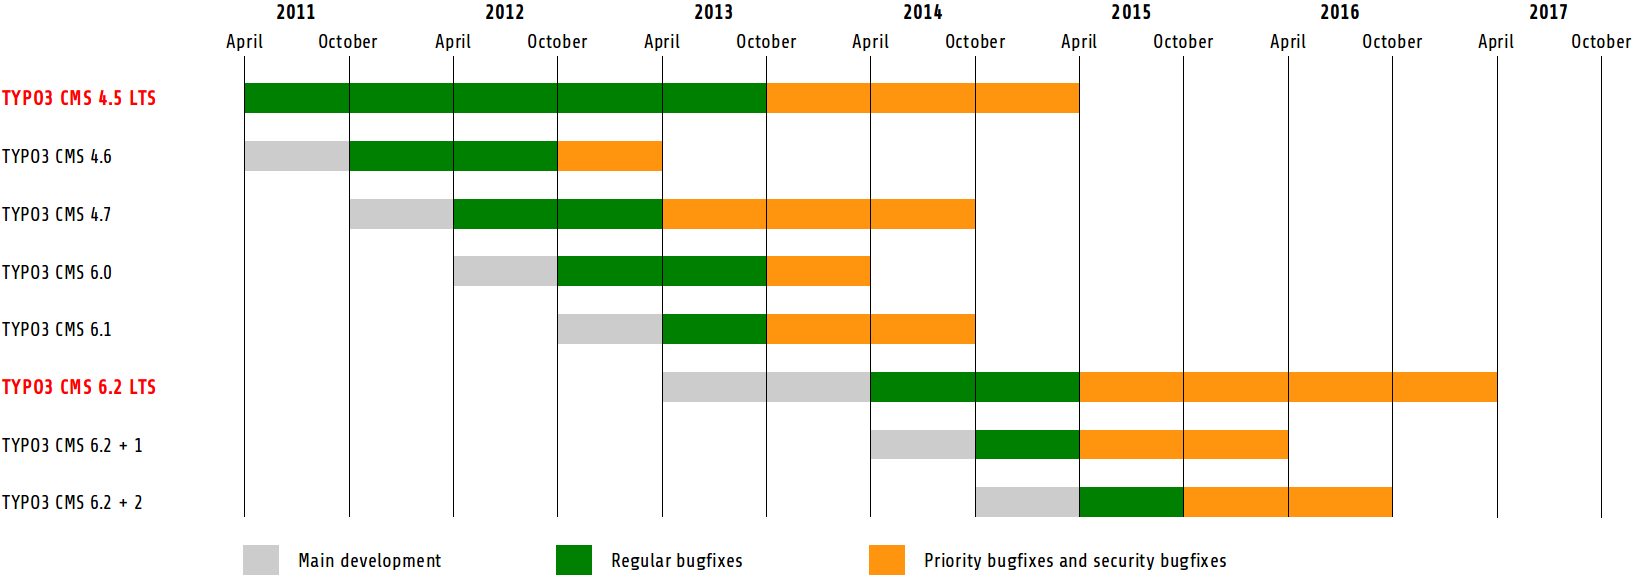
\includegraphics[width=0.99\linewidth]{Images/Introduction/ReleaseAgenda.png}
	\end{figure}

\end{frame}

% ------------------------------------------------------------------------------

